%%
%% getstart.tex -- Flight Gear documentation: Installation and Getting Started
%% Chapter file
%%
%% Written by Michael Basler, started September 1998.
%%
%% Copyright (C) 2002 Michael Basler (pmb@epost.de)
%%
%%
%% This program is free software; you can redistribute it and/or
%% modify it under the terms of the GNU General Public License as
%% published by the Free Software Foundation; either version 2 of the
%% License, or (at your option) any later version.
%%
%% This program is distributed in the hope that it will be useful, but
%% WITHOUT ANY WARRANTY; without even the implied warranty of
%% MERCHANTABILITY or FITNESS FOR A PARTICULAR PURPOSE.  See the GNU
%% General Public License for more details.
%%
%% You should have received a copy of the GNU General Public License
%% along with this program; if not, write to the Free Software
%% Foundation, Inc., 675 Mass Ave, Cambridge, MA 02139, USA.
%%
%% $Id: landing.tex,v 0.5 2002/15/02 michael
%% (Log is kept at end of this file)

%%%%%%%%%%%%%%%%%%%%%%%%%%%%%%%%%%%%%%%%%%%%%%%%%%%%%%%%%%%%%%%%%%%%%%%%%%%%%%%%%%%%%%%%%%%%%%%
\chapter{Landing: Some further thoughts before leaving the plane\label{landing}}
%%%%%%%%%%%%%%%%%%%%%%%%%%%%%%%%%%%%%%%%%%%%%%%%%%%%%%%%%%%%%%%%%%%%%%%%%%%%%%%%%%%%%%%%%%%%%%%
\markboth{\thechapter.\hspace*{1mm}
LANDING}{\thesection\hspace*{1mm} THOSE, WHO DID THE WORK}


%%%%%%%%%%%%%%%%%%%%%%%%%%%%%%%%%%%%%%%%%%%%%%%%%%%%%%%%%%%%%%%%%%%%%%%%%%%%%%%%%%%%%%%%%%%%%%%
\section{A not so Short \Index{History} of \FlightGear{}}
%%%%%%%%%%%%%%%%%%%%%%%%%%%%%%%%%%%%%%%%%%%%%%%%%%%%%%%%%%%%%%%%%%%%%%%%%%%%%%%%%%%%%%%%%%%%%%%
The \FlightGear{} project goes back to a discussion among a group of net citizens in 1996 resulting in
a proposal written by David Murr\index{Murr, David} who, unfortunately, dropped out of
the project (as well as the net) later. The original \Index{proposal} is still available
from the \FlightGear{} web site and can be found under
 \medskip

\web{http://www.flightgear.org/proposal-3.0.1}.
 \medskip

\noindent
 Although the names of the people and several of the details have changed over time,
the spirit of that proposal has clearly been retained up to the present time.

Actual coding started in the summer of 1996 and by the end of that year essential
graphics routines were completed. At that time, programming was mainly performed and
coordinated by Eric Korpela\index{Korpela, Eric} from Berkeley University. Early code ran
under \Index{Linux} as well as under \Index{DOS}, \Index{OS/2}, \Index{Windows 95/NT},
and \Index{Sun-OS}. This was found to be quite an ambitious project as it involved, among
other things, writing all the \Index{graphics routines} in a system-independent way
entirely from scratch.

Development slowed and finally stopped in the beginning of 1997 when Eric was completing
his thesis. At this point, the project seemed to be dead and traffic on the mailing list
went down to nearly nothing.

It was Curt Olson\index{Olson, Curt} from the University of Minnesota who re-launched the
project in the middle of 1997. His idea was as simple as it was powerful: Why invent the
wheel a second time? There have been several free flight simulators\index{Flight
simulator!free} available running on \Index{workstation}s under different flavors of
\Index{UNIX}. One of these, \Index{LaRCsim} (developed by Bruce Jackson\index{Jackson,
Bruce} from NASA), seemed to be well suited to the approach. Curt took this one apart and
re-wrote several of the routines such as to make them build as well as run on the
intended target platforms. The key idea in doing so was to exploit a system-independent
graphics platform: \Index{OpenGL}.
\medskip

 \centerline{\fbox{
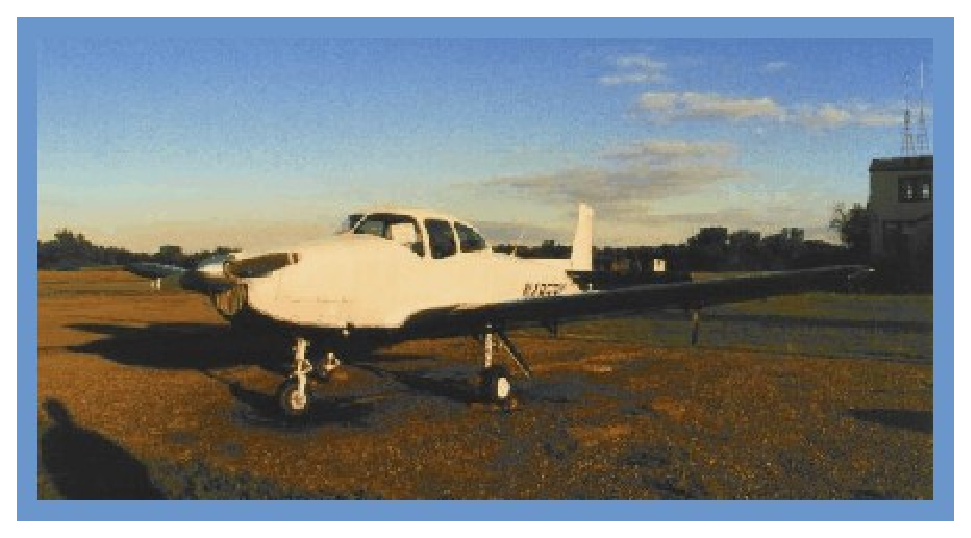
\includegraphics[clip,width=12.5cm]{navion}
}}

\smallskip
 \noindent
Fig.\,8: \textit{\Index{LaRCsim}'s \Index{Navion} is still available in \FlightGear.}
\medskip

In addition, a clever decision on the selection of the basic \Index{scenery} data was
made in the very first version. \FlightGear{} scenery is created based on satellite data
published by the \Index{U.\,S. Geological Survey}. These terrain data are available from
 \medskip

 \web{http://edcwww.cr.usgs.gov/doc/edchome/ndcdb/ndcdb.html}
 \medskip

\noindent
 for the U.S., and
  \medskip

 \web{http://edcwww.cr.usgs.gov/landdaac/gtopo30/gtopo30.html},
  \medskip

\noindent
 resp., for other countries. Those freely accessible scenery data, in
 conjunction with scenery building tools included with
 \FlightGear{}$\!$, are an important feature enabling anyone to
  create his or her own scenery.

This new \FlightGear{} code - still largely being based on the original \Index{LaRCsim}
code - was released in July 1997. From that moment the project gained momentum again.
Here are some milestones in the more recent development history:

\begin{itemize}

\item The display of sun, moon and stars have been a weak point for PC flight simulators
 for a long time. It is one of the great achievements of \FlightGear{} to include accurate modeling
 and display of sun, moon, and planets very early. The corresponding \Index{astronomy code}
 was implemented in fall 1997 by Durk Talsma\index{Talsma, Durk}.

\item Texture support\index{textures} was added by Curt
Olson\index{Olson, Curt} in spring 1998. This marked a
 significant improvement in terms of reality. You may recall that Microsoft Flight Simulator had
 non-textured scenery up until version 4.0. Some high-quality
 textures were submitted by Eric Mitchell\index{Mitchell, Eric}
  for the \FlightGear{} project.

\item A \Index{HUD} (\Index{head up display}) was added based on code
 provided by Michele America\index{America, Michele} and
 Charlie Hotch\-kiss\index{Hotchkiss, Charlie} in the fall of 1997 and was improved
 later by Norman Vine. While not generally available for real \Index{Cessna 172}, the HUD
 conveniently reports the actual flight performance of the simulation and may be of further use
 in military jets later.

\item After improving the \Index{scenery} and
\Index{texture} support  frame rate\index{frame rate} dropped down to a point where
\FlightGear{} became
 unflyable in spring 1998. This issue was resolved by exploiting hardware \Index{OpenGL}
  support, which became available at that time, and implementing
  \Index{view frustrum culling} (a rendering technique that ignores the
 part of the scenery not visible in a scene), done by Curt Olson\index{Olson, Curt}.
 Taking these measures made \FlightGear{} flyable again as long as they included a 3-D graphics board that featured
 hardware \Index{OpenGL} support. With respect to \Index{frame rate} one should keep
 in mind that the code, at present, is in no way optimized, which leaves room for further
 improvements.

\item A rudimentary \Index{autopilot} implementing heading hold was
contributed by Jeff Goeke-Smith\index{Goeke-Smith, Jeff} in April 1998. It was improved
by the addition of an altitude hold and a terrain following switch in October 1998 and
further developed by Norman Vine\index{Vine, Norman} later.

\item The basis for a menu system\index{menu} was laid based on another library,
 the Portable Library \PLIB\index{PLIB}, in June 1998. After having been idle for a time, the first
 working menu entries came to life in spring 1999.

  \PLIB{} underwent rapid development later. It has been distributed as a separate package by
  Steve Baker with a much broader range of applications in mind, since spring 1999. It
  has provided the basic graphics rendering engine for \FlightGear{} since fall 1999.

\item Friedemann Reinhard \index{Reinhard, Friedemann}
 developed early \Index{instrument panel} code, which was added in June 1998. Unfortunately,
 development of that panel slowed down later, partly because of \Index{OpenGL} compatibility
 problems. Finally, David Megginson \index{Megginson, David} decided to rebuild the panel code from scratch in January 2000. This led to a rapid
  addition of new instruments and features to the panel, resulting in nearly all main
  instruments being included until spring 2001. A handy minipanel was added in summer 2001.

\item In 1998 there was basic \Index{audio support}, i.\,e. an audio library
and some basic background engine sound. This was later integrated into the
above-mentioned portable library, \PLIB\index{PLIB}. This same library was extended to
support joystick/yoke/rudder\index{joystick} in October 1999, again marking a huge step
in terms of realism. To adapt on different joystick, configuration options were
introduced in fall 2000.

\item In September 1998 Curt Olson\index{Olson, Curt}
 succeeded in creating a complete terrain model for the U.S. The
  scenery is available worldwide via a clickable map \index{map, clickable} at:
   \medskip

\web{http://www.flightgear.org/Downloads/world-scenery.html}.
 \medskip

\item Networking/multiplayer\index{networking code}\index{multiplayer code}
 code has been integrated by Oliver Delise \index{Delise, Oliver} and Curt
Olson\index{Olson, Curt} starting fall 1999. This effort is aimed at enabling
\FlightGear{}  to run concurrently on several machines over a network, either an Intranet
or the \Index{Internet}, coupling it to a \Index{flight planner} running on a second
machine, and more. There emerged several approaches for remotely controlling FlightGear over a Network during 2001. Notably there was added support working together wirth the ''Atlas'' moving map program. Besides, an embedded HTTP server developed late in 2001 by Curt Olson\index{Olson, Curt} can now act a property manager for external programs.

\item Christian Mayer, \index{Mayer, Christian}  together with Durk Talsma,\index{Talsma, Durk}
contributed weather code in the winter of 1999. This included \Index{clouds},
\Index{winds}, and even \Index{thunderstorms}.

\item Manually changing \Index{views} in a flight simulator is in a sense always ''unreal'' but
nonetheless required in certain situations. A possible solution was supplied by Norman
Vine\index{Vine, Norman} in the winter of 1999 by implementing code for changing views
using the mouse. Alternatively, you can use a hat switch for this purpose, today.

\item Finally, \Index{LaRCsim}s \Index{Navion} was replaced as the default aircraft
 when the \Index{Cessna 172} was stable enough in February 2000 - a move most users will welcome. There are now several \Index{flight model} options to choose from at runtime: a modified and improved LaRCsim \Index{Cessna 172} developed by Tony Peden\index{Peden, Tony}, Jon Berndt's
\index{Berndt, Jon, S.} \Index{X15}, and Christian Mayer's \index{Mayer, Christian} hot
air balloon. Jon Berndt\index{Berndt, Jon, S.} has invested a lot of time in a more
realistic and versatile flight model with a more powerful aircraft configuration method.
\JSBSim, as it has come to be called, may eventually replace LaRCsim as the default
flight dynamics model (FDM), and it is planned to include such features as fuel slosh
effects, turbulence, complete flight control systems, and other features not often found
all together in a flight simulator. As an alternative, Andy Ross\index{Ross, Andy} added another flight dynamics model called \YASim{} (Yet Another Flight Dynamics Simulator) which aims at simpliciy of use, by the end of 2001. This one bought us flight modles for a 747, an A4, and a DC-3.

\item The scenery was further improved by adding geographic features including lakes, rivers,
and coastlines later, an effort still going on. Since the end of 2000, there was again
stronger focus on scenery. Textured runways were added by Dave Cornish\index{Cornish,
Dave} in spring 2001. Light textures add to the visual impression at night. To cope with
the constant growth of scenery data, a binary scenery format was introduced in spring
2001. 

\item A fully operational radio stack and working radios were added to the panel by Curt
Olson\index{Olson, Curt} in spring 2000. A huge database of Navaids contributed by Robin
Peel allows IFR navigation since then.

\item A \Index{property manager} was implemented by David Megginson\index{Megginson, David} in
fall 2000. It allows parsing a file called \texttt{.fgfsrc}\index{.fgfsrc} under
UNIX/Linux and \texttt{system.fgfsrc}\index{system.fgfsrc} under Windows for input
options. This plain ASCII file has proven useful in submitting the growing number of
input options, and notably the \Index{joystick settings}. This has proven a useful
concept, and joystick, keyboard, and panel settings are no longer hard coded but set
using *.xml files since spring 2001 thanks to work mainly by David Megginson and John
Check.\index{Check, John}

\item There was support added for static objects to the scenery in 2001, which permits placing buildung, static planes, trees and so on in the scenery. However, despite a few profs systematic includion of these landmarks is still missing.

\item There was basic ATC support added in fall 2001 by David Luff\index{Luff, David}. This is not yet fully implemented, but displaying ATIS messages is already possible.

\item A magneto switch with proper functions was added at the end of 2001 by John Check\index{Check, John} and David Megginson.\index{Megginson, David}. Actually, several panels were vastly improved during 2001 by John and others.
\end{itemize}

During development there were several code reorganization efforts. Various code
subsystems were moved into packages. As a result, presetnly code is organized as follows:
\medskip

The base of the graphics engine is \textbf{\Index{OpenGL}}, a platform independent
graphics library. Based on \Index{OpenGL}, the Portable Library \PLIB{}\index{PLIB}
provides basic rendering, audio, joystick etc. routines. Based on \PLIB\index{PLIB} is
\SimGear{}\index{SimGear}, which includes all of the basic routines required for the
flight simulator as well as for building scenery. On top of \SimGear{}\index{SimGear}
there are (i) \FlightGear{}\index{FlightGear} (the simulator itself), and (ii)
\TerraGear{}\index{TerraGear}, which comprises the scenery building tools.

This is by no means an exhaustive history and most likely some people who have made
important contributions have been left out. Besides the above-named contributions there
was a lot of work done concerning the internal structure by: Jon S. Berndt\index{Berndt,
Jon, S.}, Oliver Delise, \index{Delise, Oliver} Christian Mayer, \index{Mayer, Christian}
Curt Olson,\index{Olson, Curt} Tony Peden, \index{Peden, Tony} Gary R. Van
Sickle\index{van Sickle, Gary, R.}, Norman Vine\index{Vine, Norman}, and others. A more
comprehensive list of contributors can be found in Chapter \ref{landing} as well as in
the \texttt{Thanks} file provided with the code. Also, the \FlightGear{}
Website\index{FlightGear Website} contains a detailed history worth reading of all of the
notable development milestones at
 \medskip

 \web{http://www.flightgear.org/News/}

%%%%%%%%%%%%%%%%%%%%%%%%%%%%%%%%%%%%%%%%%%%%%%%%%%%%%%%%%%%%%%%%%%%%%%%%%%%%%%%%%%%%%%%%%%%%%%%
\section{Those, who did the work}\index{contributors}
%%%%%%%%%%%%%%%%%%%%%%%%%%%%%%%%%%%%%%%%%%%%%%%%%%%%%%%%%%%%%%%%%%%%%%%%%%%%%%%%%%%%%%%%%%%%%%%

Did you enjoy the flight? In case you did, don't forget those who devoted hundreds of
hours to that project. All of this work is done on a voluntary basis within spare time,
thus bare with the \Index{programmers} in case something does not work the way you want
it to. Instead, sit down and write them a kind (!) mail proposing what to change.
Alternatively, you can subscribe to the \FlightGear{} \Index{mailing lists} and
contribute your thoughts there. Instructions to do so can be found at
 \medskip

 \web{http://www.flightgear.org/mail.html}.
  \medskip

\noindent
 Essentially there are two lists, one of which being mainly for the developers
and the other one for end users. Besides, there is a very low-traffic list for
announcements.
\medskip

 \noindent
The following names the people who did the job (this information was essentially taken
from the file \texttt{Thanks} accompanying the code).
 \medskip

\noindent \textbf{A1 Free Sounds}\index{A1 Free Sounds} (\mail{techie@mail.ev1.net})\\
   Granted permission for the flightgear project to use some of the sound effects from their  
   site. Homepage under   
   \medskip
   
   \href{http://www.a1freesoundeffects.com/}{http://www.a1freesoundeffects.com/}
   \medskip

\noindent \textbf{Raul Alonzo}\index{Alonzo, Raul} (\mail{amil@las.es})\\
   Mr. Alonzo is the
 author of Ssystem and provided his kind permission for using the moon texture.
 Parts of his code were used as a template when adding the texture.
  Ssystem Homepage can be found at:
   \medskip

  \href{http://www1.las.es/~amil/ssystem/}{http://www1.las.es/$\tilde{~~}$amil/ssystem/}.
 \medskip

 \noindent \textbf{Michele America}\index{America, Michele}
(\mail{nomimarketing@mail.telepac.pt})\\
  Contributed to the \Index{HUD} code.
 \medskip

\noindent \textbf{Michael Basler}\index{Basler, Michael} (\mail{pmb@epost.de})\\
 Author of Installation and Getting Started. Flight Simulation Page at
  \medskip

 \web{http://www.geocities.com/pmb.geo/flusi.htm}
\medskip

\noindent \textbf{Jon S. Berndt}\index{Berndt, Jon, S.} (\mail{jsb@hal-pc.org})\\
 Working on a complete C++ rewrite/reimplimentation of the core \Index{FDM}.
  Initially he is using X15 data to test his code, but once things are
  all in place we should be able to simulate arbitrary aircraft. Jon
  maintains a page dealing with Flight Dynamics at:
   \medskip

  \web{http://jsbsim.sourceforge.net}
   \medskip

\noindent
  Special attention to X15 is paid in separate pages on this site. Besides, Jon
  contributed via a lot of suggestions/corrections to this Guide.
\medskip

\noindent \textbf{Paul Bleisch}\index{Bleisch, Paul} (\mail{pbleisch@acm.org})\\
  Redid the debug system so that it would be much more
  flexible, so it could be easily disabled for production system, and
  so that messages for certain subsystems could be selectively
  enabled. Also contributed a first stab at a config file/command line parsing
  system.
 \medskip


\noindent \textbf{Jim Brennan}\index{Brennan, Jim} (\mail{jjb@kingmont.com})\\
  Provided a big chunk of online space to store USA scenery for \FlightGear{}$\!$.
 \medskip

\noindent \textbf{Bernie Bright}\index{Bright, Bernie}
(\mail{bbright@bigpond.net.au})\\
  Many C++ style, usage, and implementation improvements, STL
  portability and much, much more. Currently he is trying to create a BeOS
  port. Added threading support and a threaded tile pager.
 \medskip

\noindent \textbf{Bernhard H. Buckel}\index{Buckel, Bernhard}
(\mail{buckel@mail.uni-wuerzburg.de})\\
  Contributed the README.Linux.  Contributed several sections to earlier versions of
 Installation and Getting Started.
 \medskip

\noindent \textbf{Gene Buckle}\index{Buckle, Gene} (\mail{geneb@deltasoft.com})\\
  A lot of work getting \FlightGear{} to compile with the \Index{MSVC}++
  compiler. Numerous hints on detailed improvements.
 \medskip


\noindent \textbf{Ralph Carmichael}\index{Carmichael, Ralph} (\mail{ralph@pdas.com})\\
  Support of the project. The Public Domain Aeronautical Software web site at
\medskip

\web{http://www.pdas.com}
 \medskip

 \noindent
 has the PDAS CD-ROM for sale containing great programs for astronautical engineers.

\noindent \textbf{Didier Chauveau}\index{Chauveau, Didier}
(\mail{chauveau@math.univ-mlv.fr})\\
  Provided some initial code to parse the 30 arcsec DEM files found at:
   \medskip

  \web{http://edcwww.cr.usgs.gov/landdaac/gtopo30/gtopo30.html}.
 \medskip

\noindent \textbf{John Check}\index{Check, John} (\mail{j4strngs@rockfish.net})\\
 John maintains the base package CVS repository. He contributed cloud textures, wrote an excellent Joystick howto as well as a panel
 howto. Moreover, he contributed new instrument panel configurations. \FlightGear{}
 page at
 \medskip

 \web{http://rockfish.net/fg/}.
 \medskip

\noindent \textbf{Dave Cornish}\index{Cornish, Dave} (\mail{dmc@halcyon.com})\\
 Dave created new cool runway textures.
 \medskip

\noindent \textbf{Oliver Delise} \index{Delise, Oliver} (\mail{delise@mail.isis.de})\\
 Started a FAQ, Documentation, Public relations. Working on adding some
  networking/multi-user code.\index{networking code} Founder of the FlightGear MultiPilot
  Project at
   \medskip

  \href{http://www.isis.de/members/~odelise/progs/flightgear}{http://www.isis.de/members/$\tilde{~~}$odelise/progs/flightgear}.
\medskip

\noindent \textbf{Jean-Francois Doue}\index{Doue, Jean-Francois}\\
  Vector 2D, 3D, 4D and Matrix 3D and 4D inlined C++ classes.  (Based on
  Graphics Gems IV, Ed. Paul S. Heckbert)
  \medskip

\href{http://www.animats.com/simpleppp/ftp/public_html/topics/developers.html}{http://www.animats.com/simpleppp/ftp/public\_html/topics/developers.html}.
 \medskip

\noindent \textbf{Dave Eberly} \index{Eberly, Dave} (\mail{eberly@magic-software.com})\\
  Contributed some sphere interpolation code used by Christian Mayer's
  weather data base system.  On Dave's web site there are tons of
  really useful looking code at
   \medskip

  \web{http://www.magic-software.com}.
  \medskip

\noindent \textbf{Francine Evans}\index{Evans, Francine} (\mail{evans@cs.sunysb.edu})
 \medskip

\href{http://www.cs.sunysb.edu/~evans/stripe.html}{http://www.cs.sunysb.edu/\~{}evans/stripe.html}
\medskip

  \noindent
  Wrote the GPL'd tri-striper.
 \medskip

\noindent \textbf{Oscar Everitt}\index{Everitt, Oscar} (\mail{bigoc@premier.net})\\
  Created single engine piston engine sounds as part of an F4U package
  for \Index{FS98}.  They are pretty cool and Oscar was happy to contribute
  them to our little project.
 \medskip

\noindent \textbf{Bruce Finney}\index{Finney, Bruce} (\mail{bfinney@gte.net})\\
  Contributed patches for MSVC5 compatibility.
 \medskip

\noindent \textbf{Jean-loup Gailly}\index{Gailly, Jean-loup} and \textbf{Mark
Adler}\index{Adler, Mark} (\mail{zlib@gzip.org})\\
  Authors of the \Index{zlib library}.  Used for on-the-fly compression and
  decompression routines,

  \web{http://www.cdrom.com/pub/infozip/zlib/}.
 \medskip

\noindent \textbf{Mohit Garg}\index{Garg, Mohit}
(\href{mailto:theprotean_1@hotmail.com}{theprotean\_1@hotmail.com})\\
 Contributed to the manual.
 \medskip

\noindent \textbf{Thomas Gellekum}\index{Gellekum, Thomas}
(\mail{tg@ihf.rwth-aachen.de})\\
  Changes and updates for compiling on \Index{FreeBSD}.
 \medskip

\noindent \textbf{Neetha Girish}\index{Girish, Neetha}
(\mail{neethagirish@usa.net})\\
  Contributed the changes for the xml configurable HUD.
 \medskip

\noindent \textbf{Jeff Goeke-Smith}\index{Goeke-Smith, Jeff}
(\mail{jgoeke@voyager.net})\\
  Contributed our first \Index{autopilot} (Heading Hold).
  Better autoconf check for external timezone/daylight variables.
 \medskip

\noindent \textbf{Michael I. Gold}\index{Gold, Michael, I.}
(\mail{gold@puck.asd.sgi.com})\\
 Patiently answered questions on \Index{OpenGL}.
 \medskip

\noindent \textbf{Habibe}\index{Habibe} (\mail{habibie@MailandNews.com})\\
 Made RedHat package building changes for SimGear.
 \medskip

\noindent \textbf{Mike Hill}\index{Hill, Mike} (\mail{mikehill@flightsim.com})\\
 For allowing us to concert and use his wonderful planes, available form
 \medskip

 \web{http://www.flightsimnetwork.com/mikehill/home.htm},

 \noindent
 for \FlightGear{}.
 \medskip

\noindent \textbf{Erik Hofman}\index{Hofman, Erik} (\mail{erik.hofman@a1.nl})\\
 Contributed SGI IRIX support and binaries.
 \medskip

\noindent \textbf{Charlie Hotchkiss}\index{Hotchkiss, Charlie}
(\mail{clhotch@pacbell.net})\\ Worked on improving and enhancing the \Index{HUD} code.
Lots of code style tips and code tweaks.
 \medskip

\noindent \textbf{Bruce Jackson}\index{Jackson, Bruce} (NASA)
(\mail{e.b.jackson@larc.nasa.gov})
 \medskip

  \web{ http://dcb.larc.nasa.gov/www/DCBStaff/ebj/ebj.html}
  \medskip

 \noindent
   Developed the \Index{LaRCsim} code under funding by NASA which we use to provide the
   flight model. Bruce has patiently answered many, many questions.
 \medskip


\noindent \textbf{Ove Kaaven} \index{Kaaven, Ove} (\mail{ovek@arcticnet.no})\\
 Contributed the Debian binary.
 \medskip

\noindent \textbf{Richard Kaszeta} \index{Kaszeta, Richard} (\mail{bofh@me.umn.edu})\\
  Contributed screen buffer to ppm screen shot routine.
  Also helped in the early development of the "altitude
  hold autopilot module"\index{autopilot} by teaching Curt Olson the basics of Control Theory
  and helping him code and debug early versions. Curt's ''Boss'' Bob Hain
 (\mail{bob@me.umn.edu}) also contributed to that.  Further details available at:
 \medskip

  \web{http://www.menet.umn.edu/~curt/fgfs/Docs/Autopilot/AltitudeHold/AltitudeHold.html}.
  \medskip

\noindent
  Rich's Homepage is at
  \medskip

  \web{http://www.menet.umn.edu/~kaszeta}.
  \medskip

\noindent \textbf{Tom Knienieder}\index{Knienieder, Tom} (\mail{tom@knienieder.com})\\
  Ported the audio library\index{audio library} first to OpenBSD and IRIX and after that to Win32.
 \medskip

\noindent \textbf{Reto Koradi}\index{Koradi, Reto} (\mail{kor@mol.biol.ethz.ch})
 \medskip

\href{http://www.mol.biol.ethz.ch/~kor}{\web{http://www.mol.biol.ethz.ch/\~{}kor}}
 \medskip

\noindent
  Helped with setting up \Index{fog effects}.
 \medskip

\noindent \textbf{Bob Kuehne}\index{Kuehne, Bob} (\mail{rpk@who.net})\\
  Redid the Makefile system so it is simpler and more robust.
 \medskip

\noindent \textbf{Kyler B Laird}\index{Laird, Kyler B.} (\mail{laird@ecn.purdue.edu})\\
 Contributed corrections to the manual.
 \medskip

\noindent \textbf{David Luff}\index{Luff, David} (\mail{david.luff@nottingham.ac.uk})\\
 Contributed heavily to the IO360 piston engine model.
 \medskip

\noindent \textbf{Christian Mayer}\index{Mayer, Christian}
(\mail{flightgear@christianmayer.de})\\
 Working on \Index{multi-lingual conversion tools} for fgfs as a demonstration of technology.
 Contributed code to read Microsoft Flight Simulator scenery textures. Christian is working on a completely new \Index{weather} subsystem.
 Donated a \Index{hot air balloon} to the project.
 \medskip

\noindent \textbf{David Megginson}\index{Megginson, David} (\mail{david@megginson.com})\\
  Contributed patches to allow mouse input to control view direction yoke.
  Contributed financially towards hard drive space for use by the
  flight gear project. Updates to README.running.
  Working on getting fgfs and ssg to work without textures.
  Also added the new 2-D panel and the save/load support.
  Further, he developed new \Index{panel} code, playing better with OpenGL, with new features.
  Developed the property manager and contributed to joystick support.
 \medskip

 \medskip

\noindent \textbf{Cameron Moore}\index{Moore, Cameron}
(\mail{cameron@unbeatenpath.net})\\
 FAQ maintainer. Reigning list administrator. Provided man pages.
 \medskip

\noindent \textbf{Eric Mitchell}\index{Mitchell, Eric} (\mail{mitchell@mars.ark.com})\\
  Contributed some topnotch scenery \Index{textures} being all original creations by him.
 \medskip

\noindent \textbf{Alan Murta}\index{Murta, Alan} (\mail{amurta@cs.man.ac.uk})
 \medskip

  \web{http://www.cs.man.ac.uk/aig/staff/alan/software/}
   \medskip

  \noindent
  Created the Generic Polygon Clipping library.
 \medskip

\noindent \textbf{Phil Nelson}\index{Nelson, Phil} (\mail{phil@cs.wwu.edu})\\
  Author of GNU dbm, a set of database routines that use extendible hashing and work
  similar to the standard UNIX dbm routines.
  \medskip

\noindent \textbf{Alexei Novikov}\index{Novikov, Alexei}
(\mail{anovikov@heron.itep.ru})\\
  Created European Scenery. Contributed a script to turn fgfs scenery into beautifully rendered
  2-D maps. Wrote a first draft of a Scenery Creation Howto.
  \medskip

\noindent \textbf{Curt Olson}\index{Olson, Curt} (\mail{curt@flightgear.org})\\
 Primary organization of the project.\\
 First implementation and modifications based on \Index{LaRCsim}.\\
 Besides putting together all the pieces provided by others mainly concentrating on the \Index{scenery subsystem} as well as the graphics stuff. Homepage at

 \web{http://www.menet.umn.edu/~curt/}
 \medskip
 
 noindent \textbf{Brian Paul}\index{Paul, Brian}\\
 We made use of his TR library and of course of Mesa:
 
 \web{http://www.mesa3d.org/brianp/TR.html}, \web{http://www.mesa3d.org}
 \medskip

\noindent \textbf{Tony Peden}\index{Peden, Tony}  (\mail{apeden@earthlink.net})\\
  Contributions on flight model development, including a LaRCsim based
  Cessna 172. Contributed to  {\JSBSim} the initial conditions code, a more complete
  standard atmosphere model, and other bugfixes/additions.
  His Flight Dynamics page can be found at:
   \medskip

  \href{http://www.nwlink.com/~apeden}{http://www.nwlink.com/$\tilde{~~}$apeden}.
  \medskip


\noindent \textbf{Robin Peel}\index{Peel, Robin} (\mail{robin@cpwd.com})\\
  Maintains worldwide airport and runway database for \FlightGear{} as well as X-Plane.
 \medskip

\noindent \textbf{Alex Perry}\index{Perry, Alex} (\mail{alex.perry@ieee.org})\\
 Contributed code to more accurately model VSI, DG, Alticude.
 Suggestions for improvements of the layout of the simulator on the mailing list
 and help on documentation.
 \medskip

\noindent \textbf{Friedemann Reinhard}\index{Reinhard, Friedemann}
(\mail{mpt218@faupt212.physik.uni-erlangen.de})\\
  Development of an early textured instrument \Index{panel}.
 \medskip

\noindent \textbf{Petter Reinholdtsen}\index{Reinholdtsen, Petter}
(\mail{pere@games.no})\\
  Incorporated the GNU automake/autoconf system (with libtool).
  This should streamline and standardize the build process for all
  UNIX-like platforms.  It should have little effect on IDE type
  environments since they don't use the UNIX make system.
 \medskip

\noindent \textbf{William Riley}\index{Riley, William} (\mail{riley@technologist.com})\\
  Contributed code to add ''\Index{brakes}''. Also wrote a patch to support a first
  joystick with more than 2 axis.
 \medskip
 
\noindent \textbf{Andy Ross}\index{Ross, Andy} (\mail{andy@plausible.org})\\
 Contributed a new configurable FDM called YASim (Yet Another Fligth Dynamics Simulator, based on geometry information rather than aerodynamic coefficients.
 \medskip

\noindent \textbf{Paul Schlyter}\index{Schlyter, Paul} (\mail{pausch@saaf.se})\\
  Provided Durk Talsma with all the information he needed to write the
  astro code. Mr. Schlyter is also willing to answer astro-related questions
  whenever one needs to.
  \medskip
  
  \web{http://welcome.to/pausch}
 \medskip

\noindent \textbf{Chris Schoeneman}\index{Schoenemann, Chris}
(\mail{crs@millpond.engr.sgi.com})\\
  Contributed ideas on audio support.
 \medskip

\noindent \textbf{Phil Schubert}\index{Schubert, Phil} (\mail{philip@zedley.com})\\
  Contributed various textures and engine modelling.
   \medskip

  \web{http://www.zedley.com/Philip/index.htm}.
  \medskip

 \noindent \textbf{Jonathan R Shewchuk}\index{Shewchuk, Jonathan}
(\mail{Jonathan\_R\_Shewchuk@ux4.sp.cs.cmu.edu})\\
  Author of the Triangle\index{triangle program} program.  Triangle
  is used to calculate the  Delauney triangulation of our irregular terrain.
 \medskip

\noindent \textbf{Gordan Sikic}\index{Sikic, Gordan} (\mail{gsikic@public.srce.hr})\\
  Contributed a \Index{Cherokee flight model} for \Index{LaRCsim}.  Currently is not
  working and needs to be debugged.  Use configure
  \texttt{-$ $-with-flight-model=cherokee}
  to build the cherokee instead of the \Index{Cessna}.
 \medskip

\noindent \textbf{Michael Smith}\index{Smith, Michael} (\mail{msmith99@flash.net})\\
  Contributed cockpit graphics, 3-D models, logos, and other images.
  Project Bonanza
   \medskip

  \web{http://members.xoom.com/ConceptSim/index.html}.
 \medskip

 \noindent
\noindent \textbf{Durk Talsma}\index{Talsma, Durk} (\mail{d.talsma@chello.nl})\\
  Accurate Sun, Moon, and Planets.  Sun changes color based on
  position in sky. Moon has correct phase and blends well into the
  sky.  Planets are correctly positioned and have proper magnitude. Help with time
  functions, GUI, and other things. Contributed 2-D cloud layer.\index{clouds} Website
  at
   \medskip

 \web{http://people.a2000.nl/dtals}.
 \medskip

\noindent \textbf{UIUC}\index{UIUC} - Department of Aeronautical and Astronautical
Engineering\\
  Contributed modifications to LaRCsim to allow loading of aircraft
  parameters from a file.  These modifications were made as part of an
  icing research project.
  \medskip

  Those did the coding and made it all work:\\
      Jeff Scott \mail{jscott@students.uiuc.edu}\index{Scott, Jeff}\\
      Bipin Sehgal \mail{bsehgal@uiuc.edu}\index{Sehgal, Bipin}\\
      Michael Selig \mail{m-selig@uiuc.edu}\index{Selig, Michael}
  \medskip

  Moreover, those helped to support the effort:\\
      Jay Thomas \mail{jthomas2@uiuc.edu}\index{Thomas, Jay}\\
      Eunice Lee \mail{ey-lee@students.uiuc.edu}\index{Lee, Eunice}\\
      Elizabeth Rendon \mail{mdfhoyos@md.impsat.net.co}\index{Rendon, Elizabeth}\\
      Sudhi Uppuluri \mail{suppulur@students.uiuc.edu}
  \medskip


\noindent
 \textbf{\Index{U.\,S. Geological Survey}}
  \medskip

\web{http://edcwww.cr.usgs.gov/doc/edchome/ndcdb/ndcdb.html}
 \medskip

 \noindent
  Provided geographic data used by this project.
 \medskip

\noindent \textbf{Mark Vallevand}\index{Vallevand, Mark}
(\mail{Mark.Vallevand@UNISYS.com})\\
  Contributed some METAR parsing code and some win32 screen printing routines.
\medskip

\noindent \textbf{Gary R. Van Sickle}\index{van Sickle, Gary, R.}
(\mail{tiberius@braemarinc.com})\\
  Contributed some initial \Index{GameGLUT} support and other fixes. Has done some
  interesting preliminary work on a binary file format. Check
  \medskip

 \web{http://www.woodsoup.org/projs/ORKiD/fgfs.htm}.
 \medskip

\noindent \textbf{Martin Spott}\index{Spott, Martin} (\mail{Martin.Spott@uni-duisburg.de})\\
 Co-Author of the ''Getting Started''.
\medskip

\noindent \textbf{Norman Vine}\index{Vine, Norman} (\mail{nhv@yahoo.com})\\
  Provided more numerous URL's to the ''FlightGear Community''.
  Many performance optimizations throughout the code.  Many contributions
  and much advice for the scenery generation section.  Lots of Windows
  related contributions. Contributed wgs84 distance and course routines.
  Contributed a great circle route autopilot mode based on wgs84 routines.
  Many other GUI, HUD and autopilot contributions.  Patch to allow mouse input to control view direction. Ultra hires tiled screen dumps. Contributed the initial 'goto airport' and 'reset' functions and the initial http image server code
\medskip

\noindent \textbf{Roland Voegtli}\index{Voegtli, Roland}
(\mail{webmaster@sanw.unibe.ch})\\
 Contributed great photorealistic textures.   Founder of European Scenery Project for
 X-Plane:
 \medskip

  \web{http://www.g-point.com/xpcity/esp/}
\medskip


\noindent \textbf{Carmelo Volpe}\index{Volpe, Carmelo}
(\mail{carmelo.volpe@mednut.ki.se})\\
  Porting \FlightGear{} to the \Index{Metro Works} development environment
  (PC/Mac).
 \medskip

\noindent \textbf{Darrell Walisser}\index{Walisser, Darrell}
(\mail{dwaliss1@purdue.edu})\\
 Contributed a large number of changes to porting \FlightGear{} to the Metro Works development environment (PC/Mac). Finally produced the first Macintosh port. Contributed to the Mac part of Getting Started, too.
\medskip

\noindent \textbf{Ed Williams}\index{Williams, Ed}
(\href{Ed_Williams@compuserve.com}{Ed\_Williams@compuserve.com}).\\
  Contributed magnetic variation code (impliments Nima WMM 2000).
  We've also borrowed from Ed's wonderful aviation formulary at various
  times as well. Website at
  \medskip
  \href{http://www.best.com/~williams/index.html}{http://www.best.com/$\tilde{~~}$williams/index.html},
 \medskip

 \noindent \textbf{Jean-Claude Wippler}\index{Wippler, Jean-Claude}
 (\mail{jcw@equi4.com})\\
  Author of \Index{MetaKit} - a portable, embeddible database with a portable
  data file format used in \FlightGear{}. Please see the following URL for more info:
 \medskip

  \web{http://www.equi4.com/metakit}
  \medskip

\noindent \textbf{Woodsoup Project}\index{Woodsoup}\\

\web{http://www.woodsoup.org}

While \FlightGear{} no longer uses Woodsoup servies we appreciate the support provied to our project during the time they hosted us. Once they provided computing resources and services so that the \FlightGear{} project could have a real home.


\noindent \textbf{Robert Allan Zeh}\index{Zeh, Allan} (\mail{raz@cmg.FCNBD.COM})\\
  Helped tremendously in figuring out the \Index{Cygnus} Win32 compiler and
  how to link with .dll's.  Without him the first run-able Win32
  version of \FlightGear{} would have been impossible.

%%%%%%%%%%%%%%%%%%%%%%%%%%%%%%%%%%%%%%%%%%%%%%%%%%%%%%%%%%%%%%%%%%%%%%%%%%%%%%%%%%%%%%%%%%%%%%%
\section{What remains to be done}
%%%%%%%%%%%%%%%%%%%%%%%%%%%%%%%%%%%%%%%%%%%%%%%%%%%%%%%%%%%%%%%%%%%%%%%%%%%%%%%%%%%%%%%%%%%%%%%

If you read (and, maybe, followed) this guide up to this point you may probably agree: \FlightGear{}$\!$, even in its present state, is not at all for the birds. It is
already a flight simulator which sports even several selectable flight models, several planes with panels and even a HUD, terrain scenery, texturing, all the basic controls and weather.

Despite, \FlightGear{} needs -- and gets -- further development. Except internal tweaks,
there are several fields where \FlightGear{} needs basics improvement and development. A
first direction is adding \Index{airport}s, streets, and more of those things bringing
scenery to real life and belonging to realistic airports. Another task is further
implementation of the \Index{menu system}, which should not be too hard with the basics
being working now. A lot of options at present set via command line or even during
compile time should finally make it into menu entries. Finally, \FlightGear{} lacks any
\Index{ATC} until now. 

There are already people working in all of these directions. If you're a programmer and
think you can contribute, you are invited to do so.

%%%%%%%%%%%%%%%%%%%%%%%%%%%%%%%%%%%%%%%%%%%%%%%%%%%%%%%%%%%%%%%%%%%%%%%%%%%%%%%%%%%%%%%%%%%%%%%
\subsection*{Achnowledgements}
%%%%%%%%%%%%%%%%%%%%%%%%%%%%%%%%%%%%%%%%%%%%%%%%%%%%%%%%%%%%%%%%%%%%%%%%%%%%%%%%%%%%%%%%%%%%%%%
Obviously this document could not have been written without all those contributors
mentioned above making \FlightGear{} a reality.

First, I was very glad to see Martin Spott \index{Spott, Martin} entering the documentation effort. Martin provided not only several updates and contributions (notably in the OpenGL section) on the Linux side of the project but also several general ideas on the documentation in general

Besides, I would like to say special thanks to Curt Olson,\index{Olson, Curt} whose
numerous scattered Readmes, Thanks, Webpages, and personal eMails were of special help to
me and were freely exploited in the making of this booklet.

Next, Bernhard Buckel \index{Buckel, Bernhard} wrote several sections of early versions
of that Guide and contributed at lot of ideas to it.

Jon S. Berndt \index{Berndt, Jon, S.} supported me by critical proofreading of several
versions of the document, pointing out inconsistences and suggesting improvements.

Moreover, I gained a lot of help and support from Norman Vine\index{Vine, Norman}. Maybe,
without Norman's answers I would have never been able to tame different versions of the
\Cygwin{} -- \FlightGear{} couple.

We were glad, our Mac expert Darrell Walisser \index{Walisser, Darrell} contributed the section on compiling under Mac OS X. In addition he submitted several Mac related hints and fixes.

Further contributions and donations on special points came from John Check,\index{Check,
John} (general layout), Oliver Delise \index{Delise, Oliver} (several suggestions
including notes on that chapter), Mohit Garg \index{Garg, Mohit} (OpenGL), Kyler B. Laird
\index{Laird, Kyler B.} (corrections), Alex Perry\index{Perry, Alex} (OpenGL), and Kai
Troester\index{Troester, Kai} (compile problems).

Besides those whose names got lost withing the last-minute-trouble we'd like to express our
gratitude to the following people for contributing valuable 'bug fixes' to this version of Getting Started (in random order): Cameron Moore,\index{Moore, Cameron} Melchior Franz,\index{Franz, Melchior} David Megginson,\index{Megginson, David} Jon Berndt,\index{Berndt, Jon} Alex Perry,\index{Perry, Alex}, Dave Perry,\index{Perry, Dave}, Andy Ross,\index{Ross, Andy} Erik Hofman.\index{Hofman, Erik} 

%% Revision 0.00  1998/09/08  michael
%% Initial revision for version 0.53.
%% Revision 0.01  1998/09/20  michael
%% several extensions and corrections
%% revision 0.10  1998/10/01  michael
%% final proofreading for release
%% revision 0.11  1998/11/01  michael
%% corrections on audio library, getting started
%% revision 0.12  1999/03/07  michael
%% Updated Credits
%% revision 0.20  1999/06/04  michael
%% added O. Delise, Ch. Mayer, R. Peel, R. Voegtli, several updates
%% revision 0.3 2000/03/01 michael
%% Supplemented to Jon Berndt, Oliver Delise, Christian Mayer, Durk Talsma
%% Norman Vine
%% Added David Meggison
%% Revised Acknowledgements
%% Several additions suggested and collected by Oliver Delise
%% revision 0.4 2001/05/12 michael
%% added several people entering the game during the last year
%% changed countless mail addresses
%% revision 0.5 2002/01/01 michael
%% update on history during the last year
%% added new people entering the game